% ----------------------------------------------------------
\chapter{Fundamentos}\label{cap:fundamentos}
% ----------------------------------------------------------
Neste capítulo são apresentados conceitos teóricos relacionados ao trabalho. Na seção 2.1, apresenta-se o processo de extração, transformação e carga de dados com as definições de cada etapa do processo. A seção 2.2 apresenta a plataforma de software Apache Airflow, utilizada para orquestrar fluxos de trabalho, além de seus componentes e sua interface gráfica. A seção 2.3 apresenta o conceito de dados abertos e iniciativas de transparência governamental em nível federal e municipal.
Por fim, na seção 2.4, são definidos licitações e contratos administrativos de acordo com a Lei 14.133/2021.

% ----------------------------------------------------------
\section{Extração, transformação e carga (ETL) de dados}
% ----------------------------------------------------------

Processos de extração, transformação e carga de dados são responsáveis pela coleta, extraçao, limpeza, transformação integração e carga de dados de uma ou mais
fontes para um sistema destino, tal como um \textit{data warehouse} . De acordo com \cite{vassiliadis2009extraction}, qualquer programa que filtra registros, calcula novos valores e alimenta uma fonte de dados diferente da original pode ser considerado um programa de ETL.

\cite{vassiliadis2009extraction} descrevem o fluxo de trabalho de um processo ETL como um grafo acíclico direcionado, no qual as tarefas executadas são análogas aos nodos do grafo e as relações entre entradas e saídas são análogas às arestas do grafo.

\begin{figure}[htb]
	\caption{\label{fig:Fig_1}Exemplo de fluxo de trabalho ETL.}
	\begin{center}
		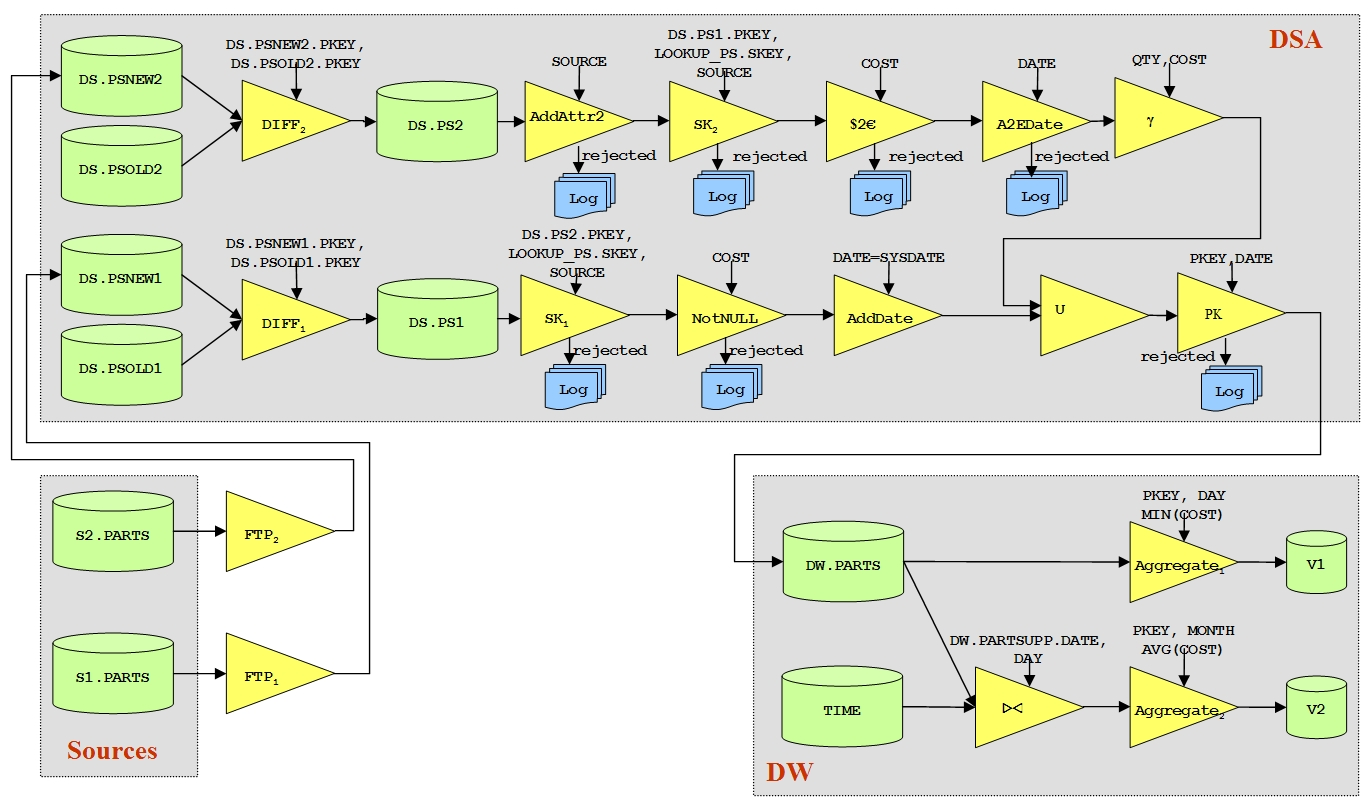
\includegraphics[scale=0.32]{images/etl.png}
	\end{center}
	\fonte{\cite{vassiliadis2009extraction}}
\end{figure}

A primeira etapa do processo ETL é a extração. Nesta, dados são obtidos de fontes, que podem estar no formato de documentos de texto, planilhas, páginas da web ou streaming. Geralmente, busca-se extrair apenas os dados que foram inseridos ou atualizados após a última execução do processo.

A segunda etapa é a transformação. Esta etapa envolve a normalização, formatação, padronização e enriquecimento de dados visando resolver problemas em nível de esquema (conflitos de nomeação de objetos ou diferenças na estruturação de dados entre fontes e o \textit{data warehouse}) e em nível de registro (registros duplicados, contraditórios, ou com referências temporais diferentes).

A terceira e última etapa é a carga. Os dados transformados são carregados nas tabelas apropriadas do \textit{data warehouse}, onde servirão como base para processos de análise, visualização e apoio a tomadas de decisões.

% ----------------------------------------------------------
\section{Apache Airflow}
% ----------------------------------------------------------

O Apache Airflow é uma plataforma de código aberto utilizada para orquestrar e monitorar fluxos de trabalho no formato de grafos acíclicos direcionados, ou DAGs. No Airflow, os DAGs são definidos por meio de arquivos, ou \textit{scripts} na linguagem Python que descrevem as tarefas a serem executadas e as dependências entre as tarefas, além de metadados com configurações específicas. O Airflow interpreta estes \textit{scripts} e modela a estrutura das DAGs, executando as tarefas de acordo com o intervalo de tempo agendado nos metadados.

De acordo com \cite{de2021data}, o uso de código em Python para definir DAGs garante flexibilidade ao desenvolvedor, pois qualquer função implementada em Python pode ser executada pelo Airflow. Assim, é possível importar funções de bibliotecas externas e criar fluxos de trabalho altamente escaláveis que estabelecem comunicações entre diversos serviços.

\cite{de2021data} afirmam que o Airflow pode ser dividido em três componentes: (i) o escalonador, que lê os \textit{scripts} de DAGs desenvolvidos e obtém as tarefas, dependências e intervalos de execução, verifica se o intervalo de cada DAG passou e, se este for o caso, adiciona as respectivas tarefas à fila de execução, (ii) os trabalhadores, que obtêm tarefas escalonadas da fila e as executam em paralelo e (iii) o servidor \textit{web}, que fornece uma interface com representações visuais das DAGs e permite que o usuário monitore os resultados das tarefas executadas.

\begin{figure}[htb]
	\caption{\label{fig:Fig_2}Diagrama mostrando os componentes do Airflow.}
	\begin{center}
		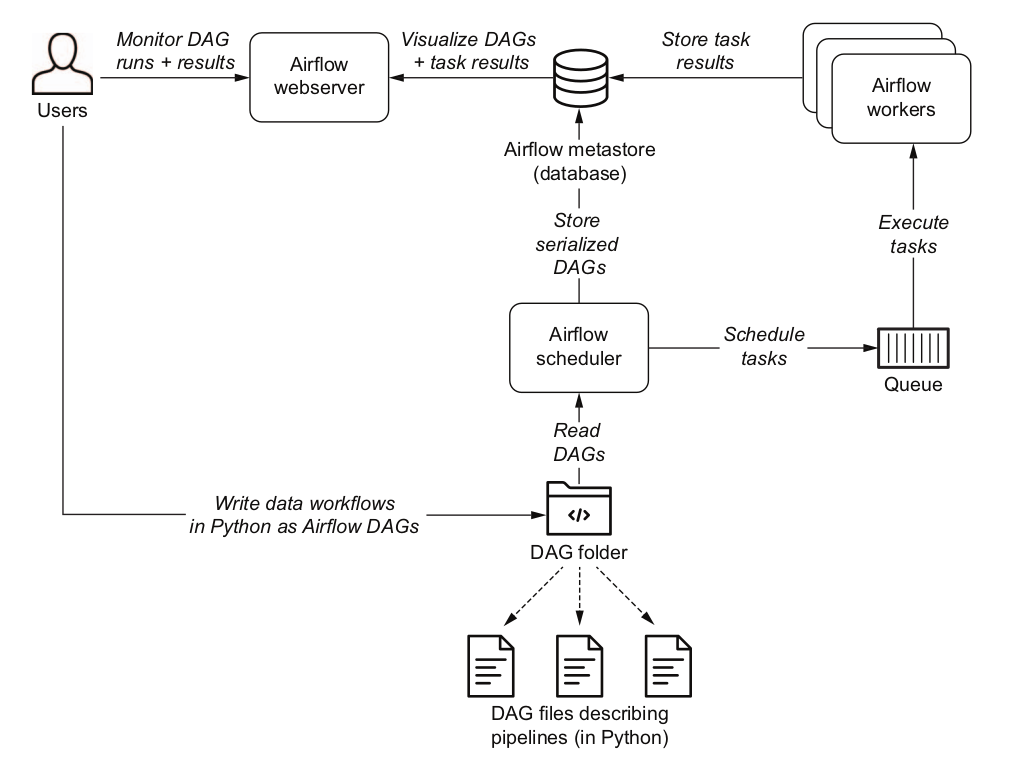
\includegraphics[scale=0.6]{images/airflow-components.png}
	\end{center}
	\fonte{\cite{de2021data}}
\end{figure}

A interface \textit{web} do Airflow oferece diferentes modos de visualização das DAGs. O modo \textit{graph view} (visualização de grafo) mostra um esquema contendo as tarefas e as respectivas dependências, enquanto o modo \textit{tree view} (visualização de árvore) mostra o histórico dos resultados das execuções das DAGs, também permitindo verificar detalhes de tarefas específicas, com indicadores de status e \textit{logs} de textos com informações referentes a possíveis erros de execução.

% ----------------------------------------------------------
\section{Transparência e dados abertos}
% ----------------------------------------------------------

\cite{possamai2020transparencia} afirmam que dados abertos governamentais são dados públicos produzidos ou curados por órgãos estatais, padronizados em formatos abertos e legíveis por máquina, como JSON ou XML, e que podem ser livremente acessados e utilizados para quaisquer finalidades. A disponibilidade de dados abertos governamentais é importante para garantir a transparência com gastos públicos, incentivar a colaboração entre o cidadão e a Administração Pública e combater a corrupção.

Segundo \cite{possamai2020transparencia}, a Lei 12.527/2011 regula o acesso às informações contidas em documentos de órgãos públicos e estabelece duas formas de transparência a serem implementadas: (i) a transparência passiva, que envolve o atendimento a solicitações de informação por meio físico ou eletrônico, e (ii) a transferência ativa, referente à divulgação de um rol mínimo de informações por parte dos órgãos independentemente de requerimento. A Lei 12.527/2011 faz referência explícita aos princípios dos dados abertos em seu texto.

De acordo com \cite{nazario2012avaliaccao}, um dos principais projetos de visualização de dados abertos governamentais é o Portal de Transparência do Governo Federal, inicialmente lançado em novembro de 2004. Em concordância com a Lei Complementar 131/09, o Portal disponibiliza informações referentes a receitas, transferências e convênios recebidos, assim como despesas envolvendo processos licitatórios, contratos e gastos com diárias.

Em relação à cidade de Florianópolis, \cite{santos2021ferramenta} afirmam que a Prefeitura Municipal regulamentou o acesso à informação pública por meio do decreto 9988/12, posteriormente instituindo o Portal de Transparência de Florianópolis por meio da Lei Municipal 9.447/14. Analogamente ao Portal de Transparência do Governo Federal, o usuário possui acesso a receitas e despesas da Prefeitura e de seus órgãos.

% ----------------------------------------------------------
\subsection{Licitações e contratos administrativos}
% ----------------------------------------------------------

\cite{tcu2023} define licitação como “o processo por meio do qual a Administração Pública convoca, sob condições estabelecidas em ato próprio (edital de licitação), interessados para apresentação de propostas relativas ao fornecimento de bens, prestação de serviços ou execução de obras”. O processo licitatório é regulamentado pela Lei 14.133/2021, cujo artigo 17 o divide em sete fases: (i) fase preparatória, (ii) divulgação do edital, (iii) apresentação de propostas e lances, (iv) julgamento, (v) habilitação, (vi) recursal e (vii) homologação.

O artigo 11 da Lei 14.133/2021 aponta como objetivos (i) garantir que seja selecionada a proposta apta a gerar o resultado de contratação mais vantajoso à Administração Pública, (ii) assegurar o tratamento isonômico e a justa competição entre os licitantes, (iii) evitar sobrepreço nas contratações e superfaturamento na execução dos contratos e (iv) incentivar a inovação e a sustentabilidade no desenvolvimento nacional.

Segundo a Lei 14.133/2021, existem cinco modalidades de licitação:
\begin{enumerate}
    \item Pregão: aquisição de bens e serviços comuns definidos pelo edital, seguindo critérios de julgamento de menor preço ou maior desconto.
    \item Concorrência: aquisição de bens e serviços especiais e de obras e serviços comuns e especiais de engenharia, utilizando critérios de julgamento de menor preço, maior desconto, melhor técnica ou conteúdo artístico, técnica e preço ou maior retorno econômico.
    \item Concurso: escolha de trabalho técnico, científico ou artístico, utilizando o critério de julgamento de melhor técnica ou conteúdo artístico e concedendo prêmio ou remuneração ao vencedor.
    \item Leilão: alienação de bens imóveis ou de bens móveis inservíveis ou legalmente apreendidos, seguindo o critério de julgamento de maior lance.
    \item Diálogo competitivo: contratação de obras, serviços e compras por meio de diálogos entre a Administração Pública e licitantes previamente selecionados, visando uma solução que atenda a uma necessidade definida.
\end{enumerate}

De acordo com \cite{tcu2023}, contratos administrativos são “aqueles firmados entre órgãos ou entidades da Administração Pública e particulares, por meio do qual se estabelece acordo de vontades, para a formação de vínculo e a estipulação de obrigações recíprocas”, que têm como objetivo principal atender a um interesse coletivo.

% \begin{figure}[htb]
% 	\caption{\label{fig:Fig_1}Elementos do trabalho acadêmico.}
% 	\begin{center}
% 		\includegraphics{images/imagem.pdf}
% 	\end{center}
% 	\fonte{Universidade Federal do Paraná (1996).}
% \end{figure}

% % ----------------------------------------------------------
% \subsection{Formatação do texto}
% % ----------------------------------------------------------

% No que diz respeito à estrutura do trabalho, recomenda-se que:
% \begin{alineas}
% 	\item o texto deve ser justificado, digitado em cor preta, podendo utilizar outras cores somente para as ilustrações;
% 	\item utilizar papel branco ou reciclado para impressão;
% 	\item  \textbf{se o trabalho for impresso}, os elementos pré-textuais devem iniciar no anverso da folha, com exceção da ficha catalográfica ou ficha de identificação da obra;
% 	\item \textbf{se o trabalho for impresso}, os elementos textuais e pós-textuais devem ser digitados no anverso e verso das folhas, quando o trabalho for impresso;

% 	\item as seções primárias devem começar sempre em páginas ímpares, quando o trabalho for impresso; e 
% 	\item deixar um espaço entre o título da seção/subseção e o texto e entre o texto e o título da subseção.
% \end{alineas}

% No \autoref{qua:Quadro_1} estão as especificações para a formatação do texto.

% \begin{quadro}[htb]
% 	\centering
% 	\caption{\label{qua:Quadro_1}Formatação do texto.}	
% 	\begin{tabular}{|l|p{11cm}|}
% 		\hline
% 		\textbf{Formato do papel} & A4.\\ \hline
% 		\textbf{Impressão}        & A norma recomenda que \textbf{caso seja necessário imprimir}, deve-se utilizar a frente e o verso da página.\\ \hline
% 		\textbf{Margens}          & Superior: 3, Inferior: 2, Interna: 3 e Externa: 2. Usar margens espelhadas quando o  trabalho for impresso.\\ \hline
% 		\textbf{Paginação}        & As páginas dos elementos pré-textuais devem ser contadas, mas não numeradas. Para trabalhos digitados somente no anverso, a numeração das páginas deve constar no canto superior direito da página, a 2 cm da borda, figurando a partir da primeira folha da  parte textual. Para trabalhos digitados no anverso e no verso, a numeração deve constar no canto superior direito, no anverso, e no canto superior esquerdo no verso.\\ \hline
% 		\textbf{Espaçamento}      & O texto deve ser redigido com espaçamento entre linhas 1,5, excetuando-se as citações de mais de três linhas, notas de rodapé, referências, legendas das ilustrações e das tabelas, natureza (tipo do trabalho, objetivo, nome da instituição a que é submetido e área de concentração), que devem ser digitados em espaço simples, com fonte menor. As referências devem ser separadas entre si por um espaço simples em branco.\\ \hline
% 		\textbf{Paginação}        & A contagem inicia na folha de rosto, mas se \textbf{insere o número da página na introdução} até o final do trabalho.\\ \hline
% 		\textbf{Fontes sugeridas} & Arial ou Times New Roman.\\ \hline
% 		\textbf{Tamanho da fonte} & \textbf{Fonte tamanho 12 para o texto}, incluindo os títulos das seções e subseções. As citações com mais de três linhas, notas de rodapé, paginação, dados internacionais de catalogação, legendas e fontes das ilustrações e das tabelas devem ser de tamanho menor. Adotamos, neste \textit{template} \textbf{fonte tamanho 10}.\\ \hline
% 		\textbf{Nota de rodapé}   & Devem ser digitadas dentro da margem, ficando separadas por um espaço simples por entre as linhas e por filete de 5 cm a partir da margem esquerda. A partir da segunda linha, devem ser alinhadas embaixo da primeira letra da primeira palavra da primeira linha.\\ \hline
% 	\end{tabular}
% 	\fonte{\textcite{NBR14724:2011}.}
% \end{quadro}

% % ----------------------------------------------------------
% \subsubsection{As ilustrações}
% % ----------------------------------------------------------

% Independentemente do tipo de ilustração (quadro, desenho, figura, fotografia, mapa, entre outros), a sua identificação aparece na parte superior, precedida da palavra designativa. 

% \begin{citacao}
% 	Após a ilustração, na parte inferior, indicar a fonte consultada (elemento obrigatório, mesmo que seja produção do próprio autor), legenda, notas e outras informações necessárias à sua compreensão (se houver). A ilustração deve ser citada no texto e inserida o mais próximo possível do texto a que se refere. \cite[p. 11]{NBR14724:2011}.
% \end{citacao}

% % ----------------------------------------------------------
% \subsubsection{Equações e fórmulas}
% % ----------------------------------------------------------

% As equações e fórmulas devem ser destacadas no texto para facilitar a leitura.  Para numerá-las, usar algarismos arábicos entre parênteses e alinhados à direita. Pode-se adotar uma entrelinha maior do que a usada no texto \cite{NBR14724:2011}.

% Exemplos, \autoref{eq:Eq_1} e \autoref{eq:Eq_2}.

% \begin{equation}\label{eq:Eq_1}
% \gls{C} = 2 \gls{pi} \gls{r}
% \end{equation}

% \begin{equation}\label{eq:Eq_2}
% \gls{A} = \gls{pi} \gls{r}^2
% \end{equation}

% % ----------------------------------------------------------
% \subsubsubsection{Exemplo tabela}
% % ----------------------------------------------------------

% De acordo com \textcite{ibge1993}, tabela é uma forma não discursiva de apresentar informações em que os números representam a informação central. Ver \autoref{tab:Tab_1}.

% \begin{table}[htb]
% 	\ABNTEXfontereduzida
% 	\caption{\label{tab:Tab_1}Médias concentrações urbanas 2010-2011.}
% 	\begin{tabular}{@{}p{3.0cm}p{1.5cm}p{2cm}p{2.5cm}p{2.5cm}p{2.5cm}@{}}
% 		\toprule
% 		\textbf{Média concentração urbana} & \multicolumn{2}{l}{\textbf{População}} & \textbf{Produto Interno Bruto – PIB (bilhões R\$)} & \textbf{Número de empresas} & \textbf{Número de unidades locais} \\ \midrule
% 		\textbf{Nome}                      & \textbf{Total}   & \textbf{No Brasil}  &                                                   &                             & \\
% 		                      &    &    &                                                   &                             & \\
% 		Ji-Paraná (RO)                     & 116 610          & 116 610             & 1,686                                             & 2 734                       & 3 082 \\
% 		Parintins (AM)                     & 102 033          & 102 033             & 0,675                                             & 634                         & 683 \\
% 		Boa Vista (RR)                     & 298 215          & 298 215             & 4,823                                             & 4 852                       & 5 187 \\
% 		Bragança (PA)                      & 113 227          & 113 227             & 0,452                                             & 654                         & 686 \\ \bottomrule
% 	\end{tabular}
% 	\fonte{\textcite{ibge2016}.}
% \end{table}

% ----------------------------------------------------------
\section{Dados abertos de compras públicas da PMF}
% ----------------------------------------------------------

\attention{Parágrafo inicial com descrição geral}

\subsection{API compras públicas da PMF?}

O Portal de Transparência da Prefeitura Municipal de Florianópolis disponibiliza informações relacionadas a compras públicas efetuadas pela Prefeitura e as unidades gestoras que a compõem, em concordância com o princípio de dados abertos. O \textit{website} do Portal, além de mostrar listas com registros de compras, oferece uma API REST que permite ao usuário fazer requisições destes registros utilizando o formato JSON.

A API possui diversos \textit{endpoints}, dos quais são utilizados os de consulta de licitações e de contratos administrativos. O acesso a estes \textit{endpoints} é livre, sem necessidade de chave para autenticação, e retorna um arquivo JSON com as informações da compra. Em ambos os \textit{endpoints}, é possível filtrar a consulta utilizando as datas inicial e final do período de busca e o código da unidade gestora responsável.

<MÉTODO GET; PARÂMETROS>
<LINK DESCRIÇÃO APIs>

\subsection{Descrição dos dados da fonte}

% {
% 	"informacao": "Licitacao",
% 	"ultimaAtualizacao": "03/10/2023",
% 	"totalRegistros": 2,
% 	"registros": [{
% 			"registro": {
% 				"licitacao": {
% 					"numero": "100132022",
% 					"modalidade": "Pregão",
% 					"valorEstimado": "10248.25",
% 					"objetoResumido": "CONTRATAÇÃO DE SERVIÇOS DE DESENVOLVIMENTO/MANUTENÇÃO DE SOFTWARE CUSTOMIZADO PARA ARMAZENAMENTO DE DADOS PÚBLICOS PARA AUXILIAR NA TRANSPARÊNCIA MUNICIPAL.",
% 					"dataEmissao": "2022-03-09",
% 					"aberturaData": "2022-03-12",
% 					"finalidade": "Compras e Outros Serviços",
% 					"formaJulgamento": "Por item",
% 				},
% 				"unidadeGestora": {
% 					"codigo": "3",
% 					"denominacao": "Prefeitura Municipal",
% 				},
% 				"advogado": {
% 					"pessoa": {
% 						"nome": "IRINEU JOSÉ DOS PASSOS",
% 					}
% 				},
% 				"listItens": [{
% 						"numero": "2",
% 						"denominacao": "MANUTENÇÃO DO SISTEMA ELETRÔNICO DE PROTOCOLOS E SOLICITAÇÕES",
% 						"quantidade": "12.0",
% 						"unidadeMedida": "SERVIÇO",
% 						"valorUnitarioEstimado": "589.75",
% 						"situacao": "Homologado",
% 						"listVencedores": [{
% 								"fornecedor": "MR. ROBOT SISTEMAS LTDA",
% 								"quantidade": "12.0",
% 								"valorUnitario": "1829.5",
% 								"situacao": "Vencedor",
% 							}
% 						]
% 					}, {
% 						"numero": "7",
% 						"denominacao": "DESENVOLVIMENTO E MANUTENÇÃO DE APLICATIVO",
% 						"quantidade": "1.0",
% 						"unidadeMedida": "SERVIÇO",
% 						"valorUnitarioEstimado": "3500.00",
% 						"situacao": "Homologado",
% 						"listVencedores": [{
% 								"fornecedor": "EAS-MOBILE LTDA",
% 								"quantidade": "1.0",
% 								"valorUnitario": "2000.0",
% 								"situacao": "Vencedor",
% 							}
% 						]
% 					}
% 				],
% 				"listTextos": [{
% 						"denominacao": "PROCESSO LICITATÓRIO Nº 43/2022 PREGÃO ELETRÔNICO Nº 18/2022",
% 						"link": "http://localhost:8080/epublica-file-server/rest/file/public?params=dbm39a47e93a574571d88d4de62a5ef244c09d8ec1c339dcaadfcb0f34ae1fe5a4e3d21c0be7268b346c75t6h1ba80bf",
% 					}
% 				]
% 			}, { 
% 			"registro": {
% 				"licitacao": {
% 					"numero": "100082022",
% 					"modalidade": "Tomada de Preço",
% 					"valorEstimado": "20048.5",
% 					"objetoResumido": "CONTRATAÇÃO DE EMPRESA PARA A PRESTAÇÃO DE SERVIÇOS DE ENGENHARIA PARA CONCLUSÃO DA CONSTRUÇÃO DO ESPAÇO EDUCATIVO.",
% 					"dataEmissao": "2022-02-22",
% 					"aberturaData": "2022-03-23",
% 					"finalidade": "Obras e Serviços de Engenharia",
% 					"formaJulgamento": "Por item",
% 				},
% 				"unidadeGestora": {
% 					"codigo": "8",
% 					"denominacao": "Fundo Municipal de Educação do Município",
% 				},
% 				"advogado": {
% 					"pessoa": {
% 						"nome": "JUSCELINO OLIVEIRA",
% 					}
% 				},
% 				"listItens": [{
% 						"numero": "1",
% 						"denominacao": "CONTRATAÇÃO DE EMPRESA PARA PRESTAÇÃO DOS SERVIÇOS DE CONCLUSÃO DA CONSTRUÇÃO DO ESPAÇO EDUCATIVO",
% 						"quantidade": "1.0",
% 						"unidadeMedida": "SERVIÇO",
% 						"valorUnitarioEstimado": "5089.8",
% 						"situacao": "Homologado",
% 						"listVencedores": [{
% 								"fornecedor": "BOB ENGENHARIA EIRELI",
% 								"quantidade": "2.0",
% 								"valorUnitario": "1849.5",
% 								"situacao": "Vencedor",
% 							}
% 						]
% 					}
% 				],
% 				"listTextos": [{
% 						"denominacao": "EDITAL - PL08/2022 TP05/2022 - CENTRO EDUCATIVO",
% 						"link": "http://localhost:8080/epublica-file-server/rest/file/public?params=dbm39a47e93a574571d895h6e62a5ef244c09d8ec1c339dcaadfcb0f34ae1fe1ht323d21c0be7268b346c75t6h1ba80f",
% 					}
% 				],
% 				"listEmpenhos": [{
% 						"emissao": "2019-12-19",
% 						"numero": "2810",
% 						"objetoResumido": "EMPENHO REF. NOSSA AQUISIÇÃO DE MATERIAIS DESTINADOS A CONSTRUÇÃO DO ESPAÇO EDUCATIVO",
% 						"especie": "Ordinário",
% 						"categoria": "Comum",
% 						"contrato": "080/2019",
% 						"licitacao": "042/2019PP",
% 						"recursoDiaria": "null",
% 					}
% 				],
% 				"listContratos": [{
% 						"numero": "2810",
% 						"assinatura": "2019-12-19",
% 						"inicioVigencia": "2019-12-19",
% 						"vencimento": "2019-12-31",
% 						"valorTotal": "10581.65",
% 						"objetoResumido": "Aquisição de materiais destinados a melhorias no espaço educativo",
% 					}
% 				]
% 			} 
% 		}
% 	]
% }

% \subsubsection{Cabeçalho do JSON}
% \begin{longtable}{|p{4cm}|p{3cm}|p{2cm}|p{6cm}|}
% \hline
% \textbf{Nome do Campo} & \textbf{Tipo de Dado} & \textbf{Tamanho} & \textbf{Descrição} \\
% \hline
% informacao & Texto & 50 & Tipo de informação retornada pela API (exemplo: 'Licitacao' ou 'Contrato'). \\
% \hline
% ultimaAtualizacao & Data & - & Data da última atualização dos dados no formato "dd/MM/yyyy". \\
% \hline
% totalRegistros & Inteiro & - & Número total de registros retornados na consulta. \\
% \hline
% registros & Lista & - & Lista de registros (licitações ou contratos). \\
% \hline
% \end{longtable}

% \subsubsection{Tabela da licitação}
% \begin{longtable}{|p{4cm}|p{3cm}|p{2cm}|p{6cm}|}
% \hline
% \textbf{Nome do Campo} & \textbf{Tipo de Dado} & \textbf{Tamanho} & \textbf{Descrição} \\
% \hline
% numero & Texto & 15 & Número identificador da licitação. \\
% \hline
% modalidade & Texto & 50 & Modalidade da licitação (exemplo: Pregão'', Tomada de Preço''). \\
% \hline
% valorEstimado & Decimal & 10,2 & Valor estimado da licitação. \\
% \hline
% objetoResumido & Texto & 500 & Descrição resumida do objeto da licitação. \\
% \hline
% dataEmissao & Data & - & Data de emissão da licitação no formato "yyyy-MM-dd". \\
% \hline
% aberturaData & Data & - & Data de abertura da licitação. \\
% \hline
% finalidade & Texto & 100 & Finalidade da licitação (exemplo: 'Compras e Outros Serviços', 'Obras e Serviços de Engenharia'). \\
% \hline
% formaJulgamento & Texto & 50 & Forma de julgamento da licitação (exemplo: 'Por item'). \\
% \hline
% \end{longtable}

% \subsubsection{Tabela da unidade gestora}
% \begin{longtable}{|p{4cm}|p{3cm}|p{2cm}|p{6cm}|}
% \hline
% \textbf{Nome do Campo} & \textbf{Tipo de Dado} & \textbf{Tamanho} & \textbf{Descrição} \\
% \hline
% codigo & Inteiro & - & Código identificador da unidade gestora. \\
% \hline
% denominacao & Texto & 100 & Nome da unidade gestora responsável pela licitação ou contrato. \\
% \hline
% \end{longtable}

% \subsubsection{Tabela do contrato}
% \begin{longtable}{|p{4cm}|p{3cm}|p{2cm}|p{6cm}|}
% \hline
% \textbf{Nome do Campo} & \textbf{Tipo de Dado} & \textbf{Tamanho} & \textbf{Descrição} \\
% \hline
% número & Texto & 20 & Número do contrato. \\
% \hline
% assinatura & Data & - & Data da assinatura do contrato. \\
% \hline
% inicioVigencia & Data & - & Data de início da vigência do contrato. \\
% \hline
% vencimento & Data & - & Data de vencimento do contrato. \\
% \hline
% valorTotal & Decimal & 10,2 & Valor total do contrato. \\
% \hline
% objetoResumido & Texto & 255 & Descrição resumida do contrato. \\
% \hline
% \end{longtable}

% \subsubsection{Tabela do fornecedor}
% \begin{longtable}{|p{4cm}|p{3cm}|p{2cm}|p{6cm}|}
% \hline
% \textbf{Nome do Campo} & \textbf{Tipo de Dado} & \textbf{Tamanho} & \textbf{Descrição} \\
% \hline
% pessoa.nome & Texto & 100 & Nome do fornecedor contratado. \\
% \hline
% \end{longtable}

\attention{Esquema e dicionário de dados.}

%\subsection{Esquema proposto para destino} - Capítulo da proposta

% ----------------------------------------------------------
\section{Trabalhos relacionados}
% ----------------------------------------------------------

\attention{Buscar trabalhos que tenham tratado de ETL de dados abertos de transparência governamental. Tais como (Só dei um exemplo de trabalho relacionado. Você cuida da busca bibliográfica, lista de bibtex no .bib e citações.):}

\url{https://sol.sbc.org.br/index.php/sbbd_estendido}

\attention{Do you know what your senator advocates for in the committees they participate in? An LLM-based approach to topic and stance detection in parliamentary discussions
Helen Bento Cavalcanti, Claudio E. C. Campelo}

\attention{Terminar com quadro comparativo de até 10 trabalhos relacionados (nas linhas) comparados segundo critérios (nas colunas): citação, tipo e fonte dos dados, tamannho da base, tecnologia usada}




